%!TEX root = ../NCVC.tex

\subsection{機械情報詳細}

\subsubsection{基本}
\begin{minipage}[t]{0.5\textwidth}
 【\ref{sec:simulation} Gコードの加工シミュレーション】を参照して下さい.
工作機械の基本的な情報をここで設定します.
[位置決め(G0)移動速度]が設定されていないと加工時間が計算できません.
各機械の仕様を参照して下さい.
\end{minipage}
\begin{minipage}[t]{0.5\textwidth}
\vspace*{-2zh}
\begin{figure}[H]
\centering
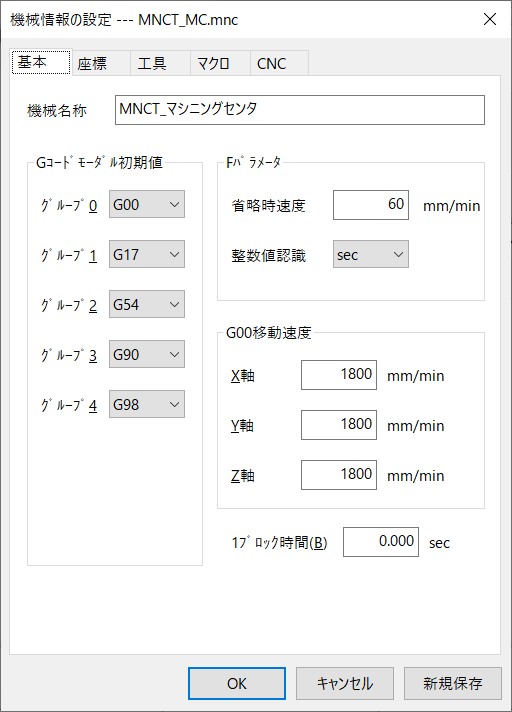
\includegraphics[scale=0.7]{No6/fig/machine1.png}
\label{fig:machine1.png}
\end{figure}
\end{minipage}

\subsubsection{座標}
\begin{minipage}[t]{0.5\textwidth}
 工作機械に登録されているワーク座標系のオフセット値を入力します.
\end{minipage}
\begin{minipage}[t]{0.5\textwidth}
\vspace*{-2zh}
\begin{figure}[H]
\centering
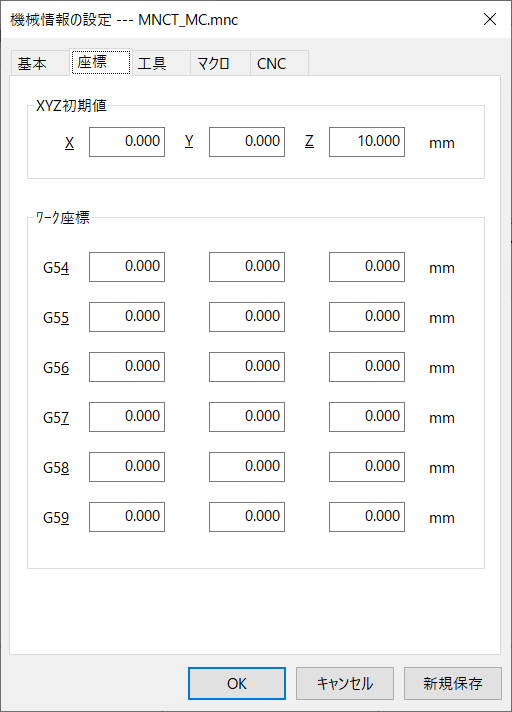
\includegraphics[scale=0.7]{No6/fig/machine2.png}
\label{fig:machine2.png}
\end{figure}
\end{minipage}

\subsubsection{工具}
\begin{minipage}[t]{0.5\textwidth}
 工具補正のための情報を登録しますが,現バージョンではサポートされていません.
\end{minipage}
\begin{minipage}[t]{0.5\textwidth}
\vspace*{-2zh}
\begin{figure}[H]
\centering
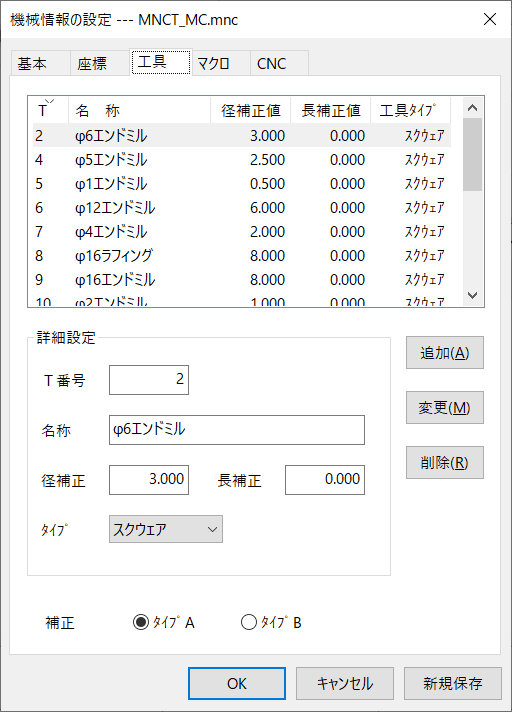
\includegraphics[scale=0.7]{No6/fig/machine3.png}
\label{fig:machine3.png}
\end{figure}
\end{minipage}

\subsubsection{マクロ}
\begin{minipage}[t]{0.5\textwidth}
 工作機械のカスタムマクロ展開用設定です.
[マクロ呼び出しコード]には正規表現で指定します.
例では G65 か G66 で P に続く数値を意味します.
[マクロ・サブプロ検索フォルダ]にはマクロやサブプロが格納されたフォルダを指定.
[マクロ変換I/F]にはマクロを展開するプログラムを指定して下さい.
NCVC単独ではマクロを展開できません.
最後に[引数]ですが,上記変換プログラムに渡す引数を指定します.
置換キーワードは以下の通りです.
\end{minipage}
\begin{minipage}[t]{0.5\textwidth}
\vspace*{-2zh}
\begin{figure}[H]
\centering
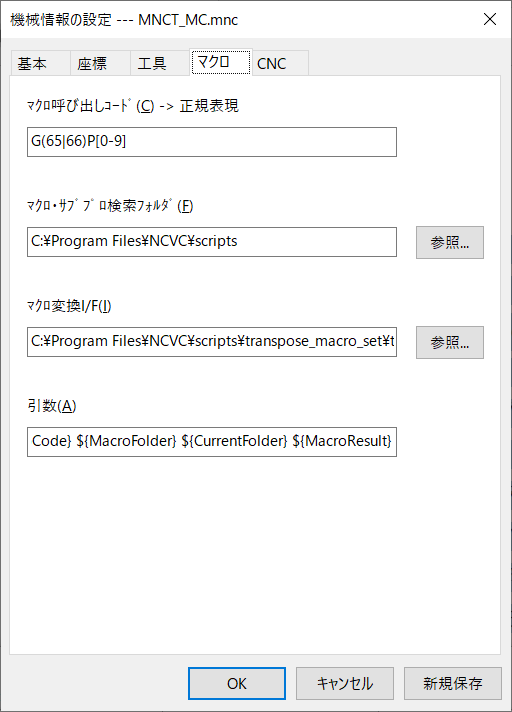
\includegraphics[scale=0.7]{No6/fig/machine4.png}
\label{fig:machine4.png}
\end{figure}
\end{minipage}

\newpage %%
 ``\,\$\{\,'' と ``\,\}\,'' で括られたとき置換キーワードと認識されます.
\begin{table}[H]
\centering
\begin{tabular}{|p{3cm}|p{10cm}|}
\hline
MacroCode     & [マクロ呼び出しコード]の正規表現にマッチしたブロック \\ \hline
MacroFolder   & [マクロ・サブプロ検索フォルダ]に置換 \\ \hline
MacroResult   & NCVCが用意する一時ファイル \\ \hline
MachineFile   & 現在選択されている機械情報ファイル \\ \hline
CurrentFolder & 現在処理中のフォルダ \\ \hline
\end{tabular}
\end{table}

\subsubsection{CNC}
\begin{minipage}[t]{0.5\textwidth}
 
\end{minipage}
\begin{minipage}[t]{0.5\textwidth}
\vspace*{-2zh}
\begin{figure}[H]
\centering
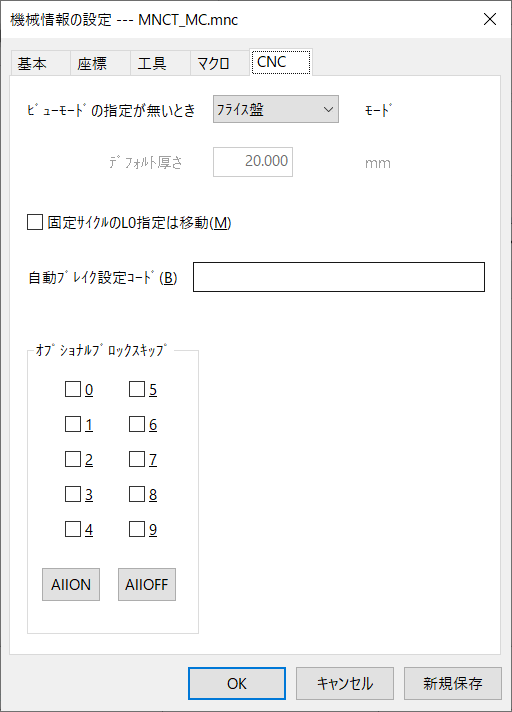
\includegraphics[scale=0.7]{No6/fig/machine5.png}
\label{fig:machine5.png}
\end{figure}
\end{minipage}
